\providecommand{\main}{..}
\documentclass[\main/main.tex]{subfiles}

\begin{document}

\chapter{Non-equilibrium Phase Transitions}
\lesson{13}{11/11/20}
What's the difference between \textit{equilibrium states} and \textit{(non-equilibrium) stationary states} NESS?

The tool that we will use in order to describe a NESS in the context of Master equations/Markov Chains is (in continuous time and discrete set of microstates $\{s_i\}$):
\begin{equation}
    \frac{\partial p(s, t)}{\partial t}=\sum_{s^{\prime}}\left[\hlc{yellow}{p\left(s^{\prime}, t\right) w_{s, s^{\prime}}}-\hlc{green}{p(s, t) w_{s^{\prime}, s}}\right]
\end{equation}
which is a differential equation for the probability $p(s,t)$ of being in state $s$ at time $t$. The $w$ are transition rates in continuous time: $w_{s,s'}$ is the transition rate from state $s'$ to $s$ and the yellow term is called \textit{gain term}, while the green one is the \textit{loss term}.

At stationarity we want that:
\begin{equation}
    \derpars{t}p=0 \quad\implies\quad \sum_{s'}\left[p(s')^s w_{s',s}-p(s)^s w_{s's}\right]\overset{!}{=} 0
    \label{eq:stat_stat}
\end{equation}
which is a relation connecting the rates of our system with stationary probability $p^s$. If (\ref{eq:stat_stat}) holds we are dealing with \textbf{steady stationary states}.

Actually we know that there is a stronger condition for equilibrium i.e. \textit{detailed balance}, where essentially every single term in the sum is equal to zero: this condition is connecting the rates of the system with the \textit{equilibrium probability} $p^{eq}$
\begin{equation}
    p(s')^{eq} w_{s',s}=p(s)^{eq} w_{s's} \,\,\, \forall \, s,s' \,\, \text{couple of states}
    \label{eq:eq_stat}
\end{equation}
and if (\ref{eq:eq_stat}) holds we are dealing with \textbf{equilibrium states}. Equilibrium states imply stationarity but not the other way round. \\

But what are the conditions for NESS? NESS are stationary states for which condition (\ref{eq:stat_stat}) holds but without detailed balance (\ref{eq:eq_stat}).

If we are in equilibrium a typical approach at fixed $T$ would be to use the Boltzmann distribution at thermodynamic equilibrium $p^{eq}(s)=\exp{-\beta E(s)/Z}$ with $Z$ known partition function in order to find the transition rates that satisfy detailed balance with the equilibrium Boltzmann distribution that we already know $p^{eq}(s)$. Practically we want to find transition rates such that:
\begin{equation}
    \frac{w_{s',s}}{w_{s,s'}}=\frac{p^{eq}(s')}{p^{eq}(s)}=\exp{-\beta[E(s')-E(s)]}
\end{equation}

An approach used to find the transition rates are Montecarlo simulations, which define rates $w_{s,s'}$ to sample the equilibrium distribution $p^{eq}(s)$: the concept is that we know the equilibrium distribution and we want to find some rates that satisfy DB and allow us to implement a numerical strategy to sample the known equilibrium distribution.
The Monte Carlo method creates a trajectory in phase space that does not correspond to real dynamics (as is the case for molecular dynamics), but the resulting visiting probability of each microstate must equal the ensemble probability. The fictitious trajectory is defined assigning the transition rates. For instance, according to the popular Metropolis algorithm, we can adopt the transition rates
\begin{equation}
    w_{s^{\prime}, s}=\min \left\{1, e^{-\beta\Delta E}\right \}
\end{equation}

Using this rates DB is satisfied for the Boltzmann distribution. \\

On the other hand, if we want to deal with NESS we don't have 'a prior' knowledge of the stationary probability distribution $p^s(s)$ and we don't have general principles like Boltzmann but what we know typically (if we want to study NESS) is that we have to assign the rates $w_{s',s}$ to define the model.

We can use for example a MC model and then we can use the stationarity condition (knowing the rates) in order to find the stationary distribution. \\

Let's deal with the following problem now:

given a set of rates $\{w_{s',s}\}$ can we decide, looking at the rates and without knowing the possible equilibrium distribution $p^{eq}(s)$, whether they are compatible with DB? Let's state a theorem which provides a sufficient and necessary condition under which a given set of rates satisfies DB (obviously specifying the equilibrium distribution):

\paragraph{Theorem}
\label{theor}
\textit{
The transition rates $w_{s^{\prime}, s}$ satisfy the detailed balance condition
$$
\frac{w_{s^{\prime}, s}}{w_{s, s^{\prime}}}=\frac{p^{\mathrm{eq}}\left(s^{\prime}\right)}{p^{\mathrm{eq}}(s)} \quad \boxed{\forall s, s^{\prime}}
$$
if and only if they satisfy the condition
\begin{equation}
    \prod_{i=1}^{N} w_{s_{i+1}, s_{i}}=\prod_{i=1}^{N} w_{s_{i-1}, s_{i}}
    \label{eq:teorema}
\end{equation}
for any set $\left(s_{1}, \ldots, s_{N}\right)$ of $N$ microstates (with the definition $s_{0}=s_{N}$ and $s_{N+1}=s_{1}$ ).} \\


Essentially the idea is that the condition of the theorem is a sort of reversibility condition on a \textit{cycle}: we can arrange our set of $N$ microstates in a circle (PBC) and the left hand side of th. \ref{theor} is the probability of going from state 1 to state 2 \dots state $s_{i}$ to $s_{i+1}$, whereas on the right hand side the we follow a clockwise order, as visualized in Figure \ref{fig:theor}a.

\begin{figure}[ht]
    \centering
    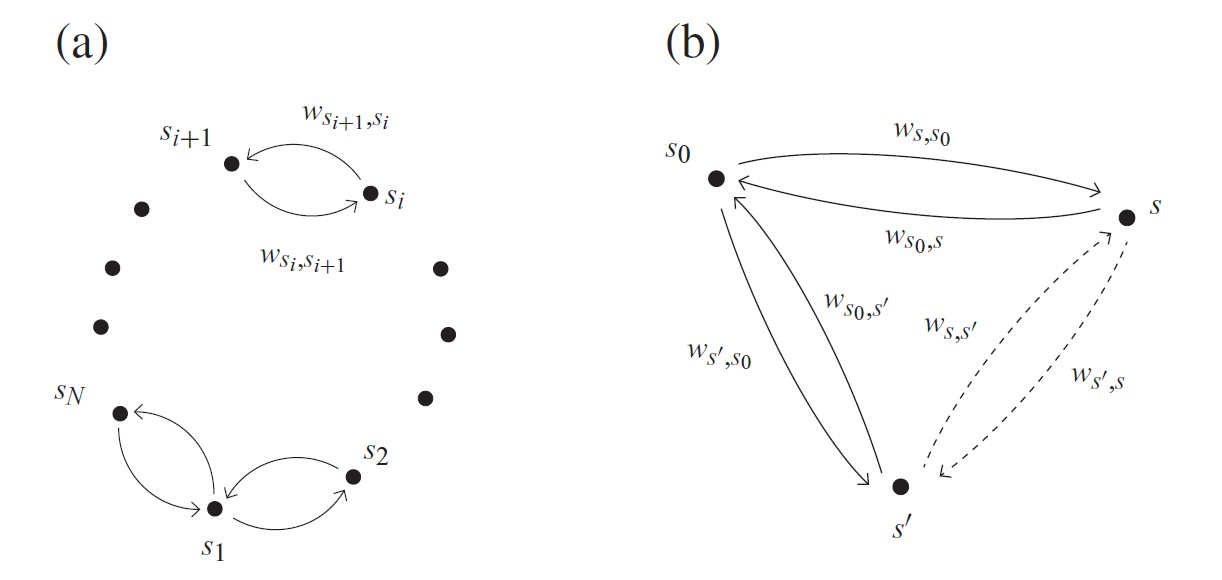
\includegraphics[width=\linewidth]{Lectures/Images/th_db.jpg}
    \caption{Graphical representation of the transition rates appearing in the proof of Theorem \ref{theor}.}
    \label{fig:theor}
\end{figure}

In other words we are stating that DB holds if for cycles in our system our rates satisfy a reversibility condition.

Intuitively, when such a reversibility condition holds, that implies that we have \textit{no (probability) currents} in the system: a current would be present if the reversibility condition wasn't satisfied\footnote{If currents are present we are in an out-of-equilibrium situation but we could be in a stationary state.}. \\

\textbf{Proof of Theorem \ref{theor}}  \\

$\boxed{\implies}$ trivial: let's take a set of $N$ microstates 
$$
\prod_{i=1}^N \frac{w_{s_{i+1},s_i}}{w_{s_{i},s_{i+1}}}\overset{DB}{=}\prod_{i=1}^N \frac{p^{eq}(s_{i+1})}{p^{eq}(s_i)}=1
$$

because since we are dealing with a cycle $p^{eq}(s_{i+1})=p^{eq}(s_i)$ and in this way we proved that the reversibility condition is satisfied. \\

$\boxed{\impliedby}$ given that, for any cycle, we have the reversibility condition let's derive DB: let's define the equilibrium distribution from the rates (it's possible to recover $p^{eq}(s)$ from normalization), such that:
\begin{equation}
\boxed{p^{\mathrm{eq}}(s) = p^{\mathrm{eq}}\left(s_{0}\right) \frac{w_{s, s_{0}}}{w_{s_{0}, s}}} \quad \forall s
\label{eq:probdistri}
\end{equation}

Notice that we chose a given 'reference state $s_0$' and this is equivalent to say that DB holds for $s,s_0\,\, \forall \,s$. 
In this case DB holds only for pairs containing $s_0$ but we can say that always: our aim is to show is that DB holds for \textit{any} possible choice $s,s'$. \\

Let's choose $s,s'\neq s_0$ choosing a cycle with three different states $s_0,s',s$ as shown in Figure \ref{fig:theor}b: let's write the reversibility condition for this cycle

$$w_{s, s_{0}} w_{s^{\prime}, s} w_{s_{0}, s^{\prime}}=w_{s^{\prime}, s_{0}} w_{s, s^{\prime}} w_{s_{0}, s},$$

which must be satisfied
because the theorem condition (reversibility for any cycle) is assumed to be true. We can rewrite it as
$$
\left(\frac{w_{s, s_{0}}}{w_{s_{0}, s}}\right) w_{s^{\prime}, s}=\left(\frac{w_{s^{\prime}, s_{0}}}{w_{s_{0}, s^{\prime}}}\right) w_{s, s^{\prime}}
$$
and let us evaluate the two fractions between parentheses using our definition of $p^{eq}(s)$
$$
\frac{p^{\mathrm{eq}}(s)}{p^{\mathrm{eq}}\left(s_{0}\right)} w_{s^{\prime}, s}=\frac{p^{\mathrm{eq}}\left(s^{\prime}\right)}{p^{\mathrm{eq}}\left(s_{0}\right)} w_{s, s^{\prime}} \implies \frac{w_{s',s}}{w_{s,s'}}=\frac{p^{eq}(s')}{p^{eq}(s)}
$$
Once we cancel $p^{\mathrm{cq}}\left(s_{0}\right)$ from both sides, the above equation proves that detailed balance between $s$ and $s^{\prime}$ is valid.

In conclusion, we have given an alternative formulation of detailed balance that involves transition rates only, so we can test if detailed balance is broken or not by checking Eq. (\ref{eq:teorema}).
\qquad \qquad \qquad\qquad\qquad \qquad \qquad \qquad \qquad  \qquad \qquad\qquad\quad  $\boxed{}$

\section{Non-equilibrium phase transitions}

We will talk about two different classes of non-equilibrium phase transitions:
\begin{itemize}
    \item \textit{Transitions with absorbing states};
    \item  \textit{Transitions in driven systems}
\end{itemize}
\subsection{Systems with absorbing states}

We call a state $s$ absorbing if we are in state $s$ and my only choice is to remain in state $s$: $w_{s,s}=1$.

If my transition rates are normalized this implies that the rate of going from $s$ to any other state $s'$ needs to be zero, $w_{s',s}=0\,\forall s'\neq s$ and also means that DB would then imply that a possible equilibrium distribution need to be zero if we are in state $s'$: $p^{eq}(s')=0\,\forall s'\neq s$.

In general if we talk about a phase transition of an absorbing state we are referring to a situation in which, by varying a control parameter, for some values of the control parameter our system is not going to the absorbing phase whereas for other values the system is actually going to the absorbing phase.

There is also a very specific value of the control parameter for which these transitions happens (from absorbing/\textit{inactive} to not absorbing/\textit{active}).

If we want to study these transitions it's clear that we can't describe them in the context of an equilibrium situation: we can describe in equilibrium only the inactive state, when the system is always in the absorbing state while the transitions to absorbing (inactive) phase take place out-of-equilibrium. \\

The typical example of phase transitions with an absorbing phase is the \textbf{directed percolation}.

\subsubsection{Isotropic percolation}

Percolation is a very interesting problem and the original inspiration used to study it explain how fluid percolates through porous mediums. Take as example the way in which American coffee is prepared, using filtered coffee: in this way the boiled water is percolating through the filter. Another example is how oil percolates through rocks in the oil extraction process or the flowing of electric currents through heterogeneous conductors.

The common point in these example is that we are dealing with heterogeneous mediums and therefore in all the modeling we are dealing with stochastic activation of \textit{percolation channel} with some probability $p, 0<p<1$. \\

Let's start discussing \textit{isotropic percolation}: we are dealing in our model with a squared lattice and each site can be either \textit{wet/active} or \textit{dry/inactive}. 

The point is that wet sites can activate/wet neighbouring sites through \textit{active bonds}. We can think of active bonds as modeling pores in our heterogeneous medium. Some pores are present connecting nearby sites, while in other situations nearby sites are not connected by a pore/active bond.

The bonds are active with probability $p$, which is our external control parameter of the percolation: what we have described until now is called \textbf{bond percolation}, because the external parameter $p$ is controlling the activation of bonds and all sites are 'potentially' active. \\

\begin{figure}[ht]
    \centering
    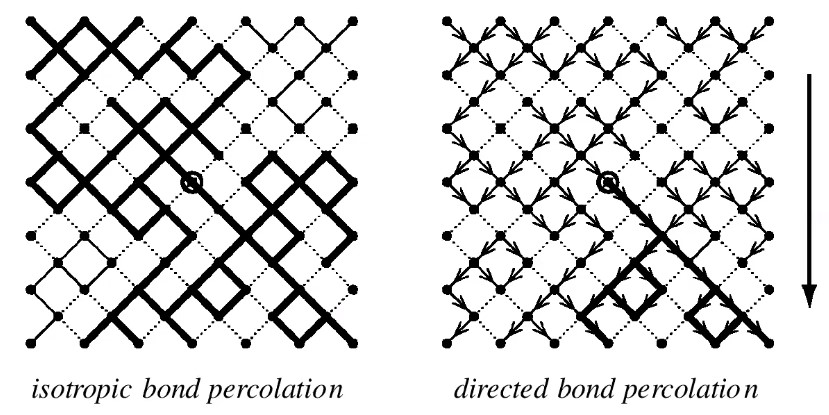
\includegraphics[width=0.87\linewidth]{Lectures/Images/percol.jpg}
    \caption{Schematic of isotropic (left) and directed (right) bond percolation. The circled point in the center is the site where
percolation originates; i.e., it is the only wet site when dynamics starts. Each bond may be active (solid line) or inactive (dashed line) and a site becomes wet if it is linked to a wet site via an active bond. Active bonds between dry sites (open circles) are thin, while active bonds between wet sites are thick. In isotropic percolation (left) the spread of wet sites proceeds isotropically, while in directed percolation (right) wetting proceeds only in the direction of the arrow. The thicker lines represent the spanning cluster.}
    \label{fig:percolation}
\end{figure}
We can also deal with \textbf{sites percolation} where sites are active with probability $p$ whereas all bonds are 'potentially' active. \\

What we want to do is to find out if there is a percolating \textit{spanning\footnote{Spanning through the whole system, from one site to the other.} cluster}: typically we will call $N$ the size of the largest active cluster and its definition is different for bond and sites percolation. It is important to stress that this definition holds for fixed system size. For bond percolation \textit{cluster size } is defined as the number of sites connected by active bonds.

Let's now consider the ratio $N/L$, where $L$ is the system size (number of sites in my lattice): when we are dealing with phase transitions is important what happens in the thermodynamic limit of system size going to infinite and therefore this is why it's relevant to consider the ratio of the size of the largest cluster over system size. Considering the thermodynamic limit what happens (ratio can't be greater than unity) is represented in Figure \ref{fig:ratio}:

\begin{figure}[ht]
    \centering
    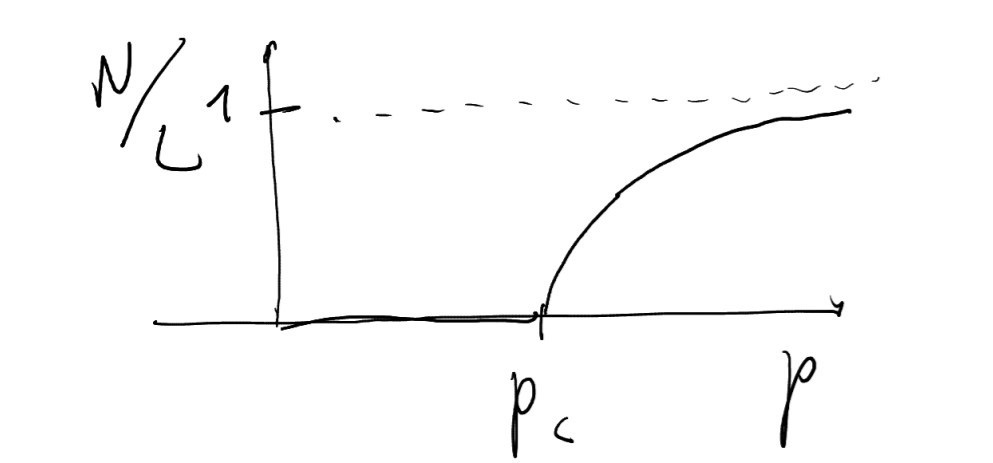
\includegraphics[width=0.8\linewidth]{Lectures/Images/limit.jpg}
    \caption{Thermodynamic limit of $N/L$; $p_c$ is the percolation threshold.}
    \label{fig:ratio}
\end{figure}

where $p_c$ is a threshold parameter, a critical value of the probability that is known as \textit{percolation threshold} below which the size of the largest active cluster does not scale linearly with the system size and above which it does.

Figure \ref{fig:ratio} is telling us that infinite size clusters appear for $p\geq p_c \,(\text{if}\, L\to\infty)$ and at the percolation threshold (which is an example of a critical point) the percolating cluster is \textit{fractal} (has fractal properties).

So far we've discussed isotropic percolation so we are still dealing with equilibrium phase transitions.

\subsubsection{Directed percolation}

In DP the preferred /allowed flow direction can be interpreted as time direction and therefore the $d+1$ dimension\footnote{We interpret the time direction as another dimension.} are meant to represent the non-equilibrium process in dimension $d$: one dimension is different from the others and it's the preferred dimension (which can be interpreted as a time).

When we talk about DP in this context we refer to it as a phase transition from a fluctuating active phase ($p>p_c$) to an inactive/absorbing phase ($p<p_c $) i.e. all sites are dry/inactive and no other sites can get wet.

Looking at Figure \ref{fig:non} we can state that at $t=0$ all sites are active and we can see what happens when times flows: when a row will be full of white dots then the system will be trapped in the absorbing phase.

\begin{figure}[ht]
    \centering
    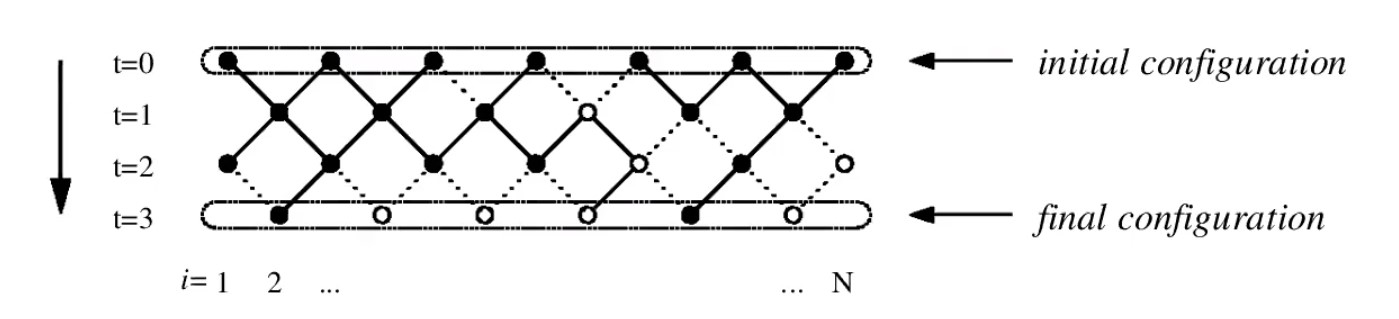
\includegraphics[width=\linewidth]{Lectures/Images/dirtime.jpg}
    \caption{Directed bond percolation in $1+1$ dimensions interpreted as a time-dependent stochastic process.
    Open (closed) bonds are indicated by solid (dashed) lines. Filled (hollow) circles denote active (inactive) sites. The configuration of the horizontal row at $t = 0$ is the initial state. Starting from a fully occupied initial state the model ‘evolves’ through intermediate configurations and reaches a final state at $t = 3$.
}
    \label{fig:non}
\end{figure}

Let's now talk about the possible dynamical processes i.e. the \textbf{stochastic rules}\marginpar{Stochastic rules}: we want to describe in detail how we can go from time $t$ to time $t+1$.

We have to give probabilities for the following transitions: what is happening at a given site at time $t+1$ is determined by the two sites that are above it at time $t$. We will use empty sites as inactive sites, full circles as active sites, dashed lines are inactive bonds, solid lines are active bonds. \\

If we have two empty sites (first image of Figure \ref{fig:tipiperc}) the site below at $t+1$ will always be empty with probability 1, it's the absorbing state. The next possible situation is the one in which a site is active and the other one inactive, with two possible outcomes: the site at $t+1$ can be either active or inactive whether the bond on the left (as represented in Figure \ref{fig:tipiperc}) is active or not. The control parameter $p$ is actually the probability of the bond being active.

The last possible configuration is the one in which both sites are active at time $t$: if both bonds are not active the site at time $t+1$ will be not active and this happens with probability $(1-p)^2$. On the other hand the site at $t+1$ can be active with probability (which can be derived through normalization) $1-(1-p)^2$ for both three sub-cases.

\begin{figure}[ht]
    \centering
    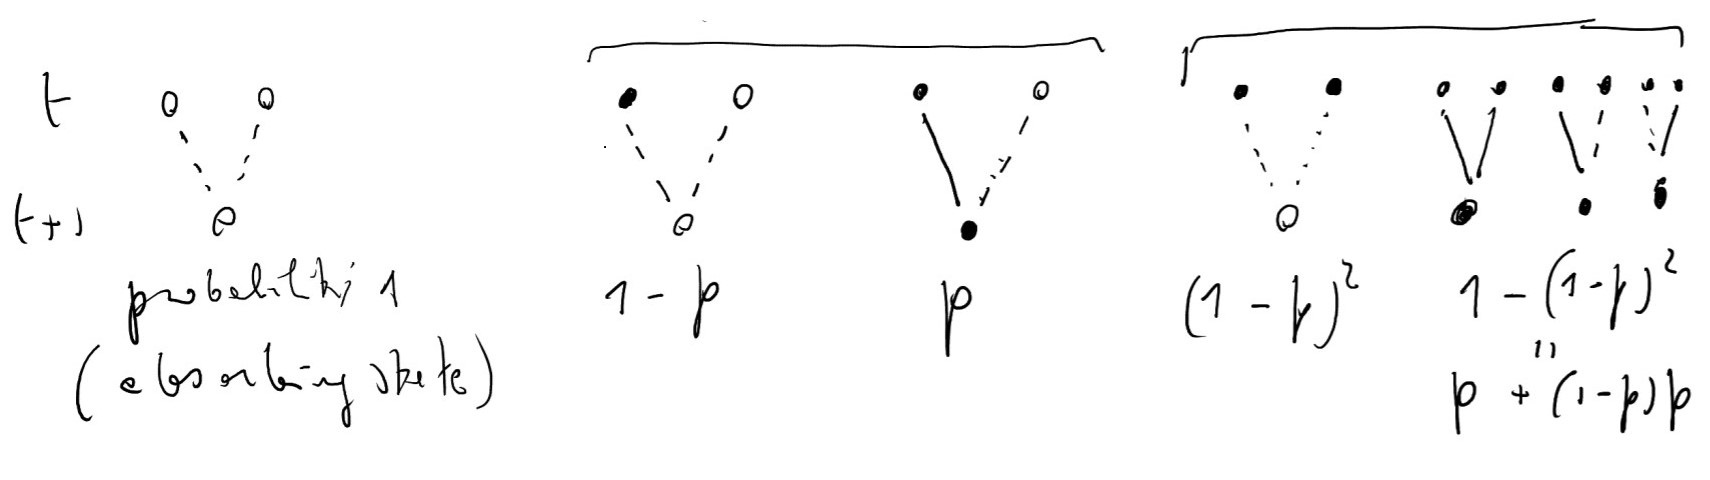
\includegraphics[width=\linewidth]{Lectures/Images/Immagine 2020-12-07 004950.jpg}
    \caption{Stochastic rules that follow the time evolution of the percolated system.}
    \label{fig:tipiperc}
\end{figure}

The rules we've just described are stochastic so in general we will talk about different realizations of the system and so given some initial conditions we can repeat the evolution several times each time choosing whether a bond is active or not with probability $p$: the outcome of different realizations could be different and then we will need to take averages over different realizations. \\

A typical order parameter is based on a Boolean variable that can be defined for each site $s_i(t)$. The index $i$ is labeling the position of different sites on the same row for a given time $1\leq i\leq L$ with $L$ system size (\# sites in a row):
\begin{numcases}{s_i(t) = \,}
1 & site $i$ is active at time $t$ \\
0 & site $i$ is inactive at time $t$
\end{numcases}

Let's now define $N(t)$ as the number of active sites at time $t$:\footnote{Shouldn't be averaged over different realizations???}
\begin{equation}
    N(t)=\sum_i s_i(t)
    \label{eq:n}
\end{equation}
One typical choice for initial conditions is to have just one site being active $s_i(0)=\delta_{i,i_0}$: knowing that the number of active sites is limited to $0\leq N(t) \leq t+1$ and so at time $t$ the number of active sites must be at most $t+1$ we can use a similar approach to the one we saw in isotropic percolation in which $p_c$ is the critical percolation threshold and for\footnote{$\mean{.}$ means average over different realizations of the stochastic process.}
\begin{numcases}{}
p<p_c \implies \mean{N(t)}\overset{t>>1}{\sim} \exp{-t/\xi_{||}}\overset{t\to\infty}{\longrightarrow} 0 &  subcritical inactive phase \\
p>p_c  \implies \mean{N(t)}\overset{t>>1}{\sim} t  & supercritical active phase \\
p=p_c \implies \mean{N(t)}\overset{t>>1}{\sim} t^\theta & critical phase
\end{numcases}
In the \textit{subcritical inactive phase }the number of active sites (asymptotically) decays exponentially in time and  we will see that this allows us to define a correlation time and for infinite times it goes to zero: we can start with some active sites but sooner or later on average no active sites survives and the system gets trapped in the inactive phase. No infinite clusters are present\footnote{With this term we are referring to 2D percolation, a spanning cluster going from top to bottom where the active sites are surviving at infinite time.}.

In the \textit{supercritical active phase} infinite clusters\footnote{Holds if the systems' size is infinite, when the number of active sites can grow indefinitely. Read on for finite sites.} exists with finite probability  and the number of active sites grows linearly with time: if we think to an initial condition with just one active site what's going on is that $N(t)$ grows with time linearly and we see a cone. The opening angle of this cone depends on $p-p_c$, on how much we are above the percolation threshold. For a  finite size system what we can state is that we have a finite density of active sites, as shown in figure \ref{fig:fig}

\begin{figure}
    \centering
    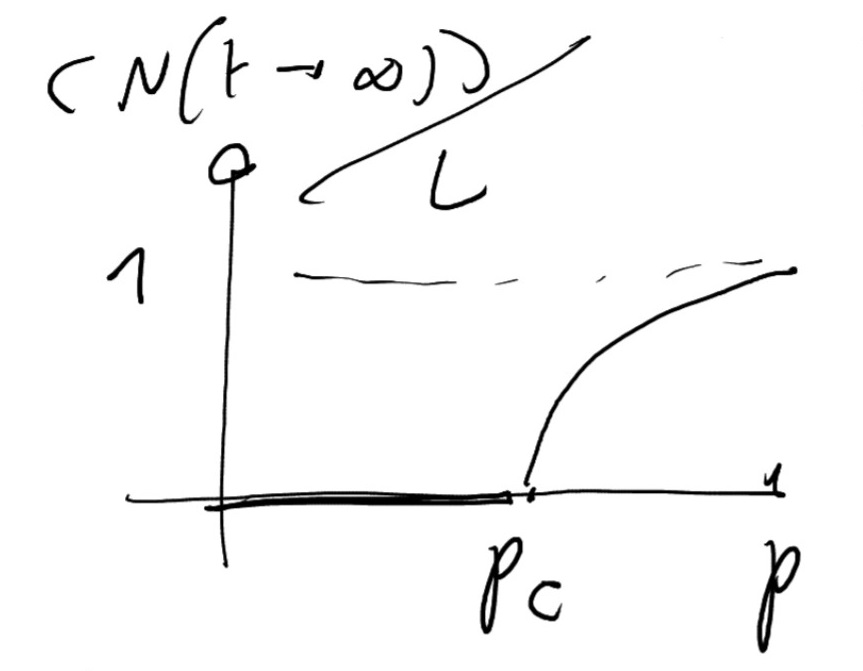
\includegraphics[width=0.35\linewidth]{Lectures/Images/aaaaa.jpg}
    \caption{Infinite time limit of the number of active sites over the system' size as a function of the percolation.}
    \label{fig:fig}
\end{figure}

In this plot we recover the same behaviour shown in Figure \ref{fig:ratio} but here we are referring to a non-equilibrium process. \\

Finally at the percolation threshold we recover a typical situation of the critical points: asymptotically the number of active sites follows a power law in time with a critical exponent $\theta$. Power laws implies that there is no characteristic length or time an essentially we can observe clusters of all sizes (or \textit{fractal clusters}) and we have scale-free behaviour.

The behaviour $\mean{N(t)}\sim t^\theta$ holds for infinite size systems. \\

Directed percolation is the analogous of the Ising model in the case of non-equilibrium phase transitions. While for $d=1,2$ we do have an analytic solution for the Ising model, for direct percolation we don't have yet an exact analytic solution, even in 1+1 (one space and one time) i.e. $d=1$: the only knowledge we have about DP is coming from numerical simulations/evidences. The critical percolation threshold is known as $p_c \simeq 0.645$ and $\theta\simeq 0.302$ and the values of the exponents are universal: we will make examples of other systems which belong to the same universality class as directed percolation implies that they show power law behaviour with the same exponent (like $\theta$) whereas the values of the control parameter at which we have a phase transition are typically non-universal (e.g. critical temperature in the Ising model). \\

\begin{figure}[ht]
    \centering
    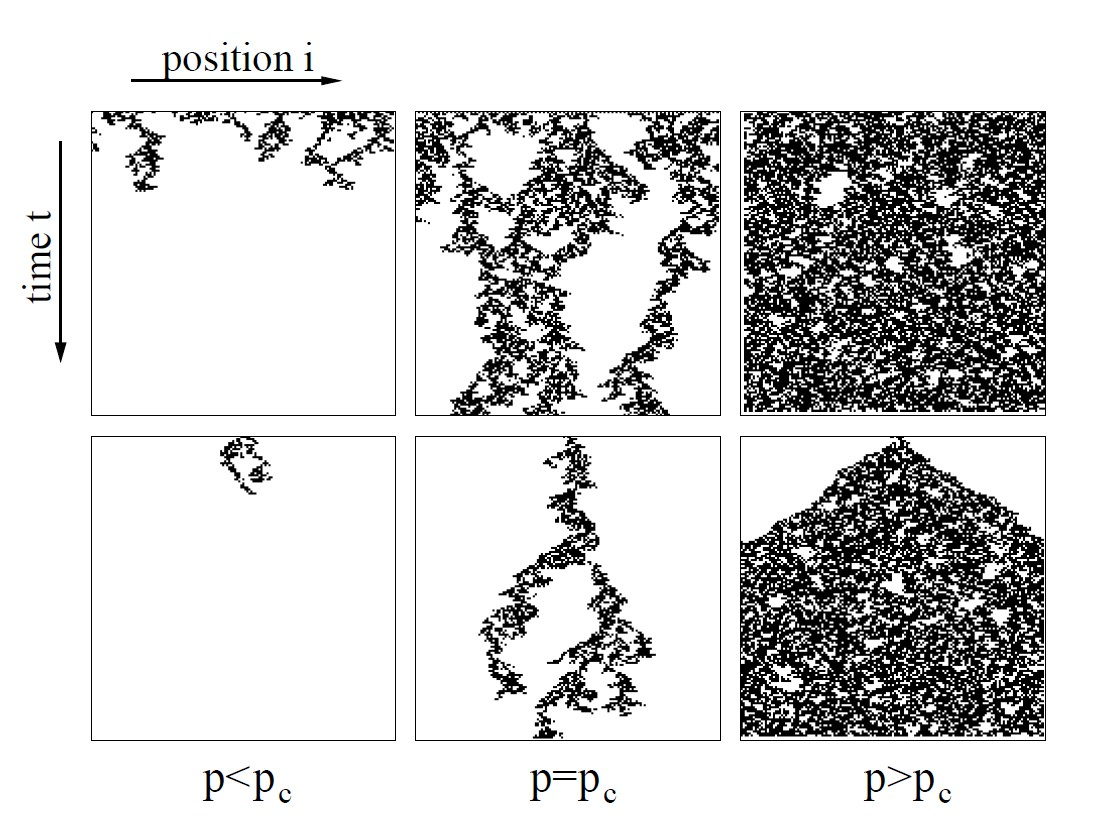
\includegraphics[width=0.7\linewidth]{Lectures/Images/experc.jpg}
    \caption{Directed bond percolation in 1+1 dimensions starting from random initial conditions (top) and
from a single active seed (bottom). Each horizontal row of pixels represents four updates. As can be seen,
critical DP is a reaction-limited process.}
    \label{fig:experc}
\end{figure}

Figure \ref{fig:experc} shows specific realizations of the system for two different types of initial conditions in the three different phases (below/at/above the transition), where $i$ labels different sites along any given row (and along a fixed time) and the time direction is the vertical one. Another typical initial condition choice (along the single initial active site at zero time, shown in the bottom row of Figure \ref{fig:experc}) is to start with a (random) fixed non-zero density of initial active sites (top row of Figure \ref{fig:experc}).

We can clearly see the behaviour previously described: in the first column active sites survive for some time but they eventually die out (no matter what the initial conditions are), above the transition we can see that the whole system is full of active sites (starting with a fixed fraction of active sites) or - starting with a single active site - we can recognize the characteristic conic shape (for a finite system) which depends on $p-p_c$ and eventually the number of active sites broads until reaches system's size $L$. The holes present in the third column of Figure \ref{fig:experc} are not fractals: at any given time we have a finite density of active sites and holes are creating and disappearing but the density of active sites is asymptotically constant.

The interesting point is at $p=p_c$ where, starting with one site or with a fraction of them, in the end we are able to get to the bottom and the active site survives at infinite time. In addition the clusters look fractalic, they look self-similar at different scales.









\end{document}